% Description: 	Electrical Power System (EPS) documenation for U-SPACE
% Author:		Morten Olsen
%
\documentclass[a4paper,11pt,titlepage]{article}
\usepackage[english]{babel}
\usepackage[margin=3cm]{geometry}
\usepackage[T1]{fontenc}
\usepackage[utf8]{inputenc}
\usepackage{lmodern}
\usepackage[sorting=none]{biblatex}
\usepackage{graphicx}
\usepackage{fancyhdr}
\usepackage[textfont={small,it},labelfont=bf,labelsep=endash]{caption}
\usepackage[table]{xcolor}
\usepackage{verbatim}
\usepackage[toc,page]{appendix}
\usepackage{amsmath}
\usepackage{multicol}	% allow multi column environemnt
\usepackage{float} % forced position of figures/tables etc.
%\usepackage{mathtools}
%\usepackage[framed,numbered]{mcode}
%\usepackage{URL}
\usepackage{acronym}
\usepackage{rotating}
\usepackage{titling}
\usepackage{bibcheck}
%\usepackage{pdfpages}
%\usepackage[pdfpagemode=FullScreen,pdfstartview=FitH,pdfborder={0 0 0},pdftitle={My report},bookmarks,pdfauthor={Morten Olsen}]{hyperref}
\usepackage{memhfixc}
%\usepackage{maplestd2e}

\graphicspath{{./figures/}}	% look for graphic files in the "figures" subfolder

\definecolor{tableshade}{HTML}{E8E8E8}
\linespread{1.3}

% define the page headers and footers
\fancyhead{}
\fancyhead[RE,RO]{\parbox[b]{10cm}{\raggedleft U-SPACE\\ \today}}
\fancyhead[LE,LO]{\parbox[b]{10cm}{\docreference \\ \title }}
\renewcommand{\headrulewidth}{0.4pt}
\fancyhfoffset{1cm}
\addtolength{\headheight}{1cm}
\fancyfoot{}
\fancyfoot[C]{\thepage}
\renewcommand{\footrulewidth}{0.4pt}

\bibliography{references} % include .bib file for citations


% PLEASE FILL IN THE RELEVANT INFORMATION BELOW:
%
\def\authors{
Zhou \textsc{Hao}\\
Dries \textsc{Agten}\\
Morten \textsc{Olsen}
}
\def\docversion{DRAFT}					% Possible versions are: DRAFT, REVIEW or RELEASED
\def\docreference{USPACE-CDR-EPS-00}	% -00 = DRAFT,  -A1 = 1st release,  -A2 = 1st release with minor updates, -B1, = 2nd release
\def\title{Critical Design Report}
\def\subtitle{Electrical Power System}



\begin{document}

\begin{titlepage}

\begin{center}


\includegraphics[width=0.6\textwidth]{figures/logo.pdf}\\[0.75cm] 

\textsc{\large Unmanned Solar Powered Airship Concept Evaluation}\\[1cm]

\line(1,0){415}\\[1mm]
\vspace{-1.0em}
\Huge \bfseries{\title}\\[2mm] 
%\
\vspace{-1.0em}
\line(1,0){415}\\[1cm]

\begin{large}
\begin{tabular}{ll}
Document Reference No.: & \docreference\\[5mm]
Document Status: & \docversion \\[1.5cm]
\end{tabular}
\end{large}

\begin{minipage}[t]{0.49\textwidth}
\begin{flushleft} \large
\emph{Authors}\\
\vspace{-1.2em}
\line(1,0){125}\\
\footnotesize{\authors}
\end{flushleft}
\end{minipage}
\begin{minipage}[t]{0.49\textwidth}
\begin{flushright} \large
\emph{Supervisors}\\
\vspace{-1.2em}
\line(1,0){125}\\
Kjell \textsc{Lundin}\\
Alf \textsc{Wikstr\"{o}m}
\end{flushright}
\end{minipage}

\vspace{1cm}

\begin{minipage}[t]{0.49\textwidth}
\begin{flushleft} \large
\emph{Project Manager}\\
\vspace{-1.2em}
\line(1,0){125}\\
Dries \textsc{Agten}
\end{flushleft}
\end{minipage}
\begin{minipage}[t]{0.49\textwidth}
\begin{flushright} \large
\emph{Quality Manager}\\
\vspace{-1.2em}
\line(1,0){125}\\
Morten \textsc{Olsen}\\[1cm]
\end{flushright}
\end{minipage}

\vfill

\begin{large}
\today \\
Lule\r{a} University of Technology \\
Rymdcampus, Kiruna, Sweden\\
\end{large}

\end{center}

\end{titlepage}

\pagestyle{plain}
\pagenumbering{roman}

\thispagestyle{plain}
\section*{Normative References}
\markboth{Normative References}{Normative References}
\addcontentsline{toc}{section}{\protect\numberline{}Normative References}
%
%
\begin{table}[H]
\centering
\caption{Normative References for this document}
\label{tab:normative_references}
\begin{minipage}{\textwidth}
\begin{tabular}{p{0.5\textwidth}p{0.3\textwidth}p{0.2\textwidth}}
\hline
\textbf{Document title} & \textbf{Doc. Ref. No.} & \textbf{Doc. status}\\
\hline
Preliminary Design Report - Electrical Power System & USPACE-PDR-EPS-A1 & Review\\
Preliminary Design Report & USPACE-PDR-A1 & Review\\
\hline
\end{tabular}\par
\vspace{-0.75\skip\footins}
\renewcommand{\footnoterule}{}
\end{minipage}
\end{table}
\thispagestyle{plain}
\chapter*{Acronyms}
\markboth{Acronyms}{Acronyms}
\addcontentsline{toc}{chapter}{\protect\numberline{}Acronyms}

\begin{multicols}{2}
\begin{acronym}
\acro{ADCS}{Attitude determination and control}
\acro{ADC}{Analog to Digital converter}
\acro{ADS}{Attitude Determination System}
\acro{BCR}{Battery Charge Regulator}
%\acro{BJT}{Bipolar Junction Transistor}
%\acro{CC}{Constant Current}
\acro{CDR}{Critical Design Review}
%\acro{CM}{Current Mode}
\acro{COTS}{Commercial Off-The-Shelf}
\acro{CPU}{Central Processing Unit}
\acro{CRC}{Cyclic Redundancy Check}
%\acro{DCM}{Discontinuous Conduction Mode}
\acro{DM}{Development Model}
\acro{DSP}{Digital Signal Processor}
\acro{ECSS}{European Cooperation for Space Standardization}
\acro{EGSE}{Electrical Ground Support Equipment}
\acro{EKF}{Extended Kalman Filter}
\acro{EMC}{Electromagnetic Compatibility}
\acro{EMI}{Electromagnetic Interference}
\acro{EPS}{Electrical Power System}
\acro{ESC}{Electronic Speed Control}
%\acro{ESR}{Equivalent Series Resistor}
\acro{ETSI}{European Telecommunications Standards Institute}
\acro{FM}{Flight Model}
%\acro{FRR}{Flight Readiness Review}
\acro{GPS}{Global Positioning System}
\acro{$I^2C$}{Inter-Integrated Circuit}
\acro{IC}{Integrated Circuit}
%\acro{IDC}{Insulation Displacment Connector}
\acro{IRF}{Swedish Institute of Space Physics}
\acro{ISE}{Integrated software environment}
\acro{ITPU}{Imaging and Tracking Payload Unit}
\acro{ITU}{International Telecommunication Union}
\acro{LDO}{Low-dropout}
\acro{LiPo}{Lithium-Polymer}
\acro{LTU}{Lule\r{a} University of Technology}
\acro{MCC}{Motor Control and Communication}
\acro{MCU}{Micro-Controller Unit}
%\acro{MEA}{Main Error Amplifier}
\acro{MGSE}{Mechanical Ground Support Equipment}
%\acro{MOSFET}{Metal-Oxide-Semiconductor Field-Effect Transistor}
%\acro{MPP}{Maximum Power Point}
\acro{MPPT}{Maximum Power Point Tracking}
%\acro{MPPTU}{Maximum Power Point Tracking Unit}
\acro{MSE}{Mechanical Structure and Envelope}
%\acro{NTC}{Negative Temperature Coefficient}
\acro{OBDH}{Onboard Data Handling}
%\acro{OpAmp}{Operational Amplifier}
\acro{OSI}{Open Systems Interconnection}
\acro{PCB}{Printed Circuit Board}
\acro{PDR}{Preliminary Design Review}
%\acro{SA}{Solar Array}
%\acro{PSA}{Pressure Sensitive Adhesive}
%\acro{PTC}{Positive Temperature Coefficient}
\acro{PWM}{Pulse Width Modulation}
%\acro{RHPZ}{Right Half Plane Zero}
\acro{RMP}{Rounds Per Minute}
\acro{SAR}{Solar Array Regulator}
\acro{SD}{Secure Digital}
\acro{SMD}{Surface-Mount Device}
\acro{SoC}{System on Chip}
\acro{SPA}{Solar Powered Airship}
\acro{SSC}{Swedish Space Corporation}
\acro{TBD}{To Be Decided}
\acro{U-SPACE}{Unmanned Solar Powered Airship Concept Evaluation}
\acro{UART}{Universal Asynchronous Receiver/Transmitter}
%\acro{UAS}{Unmanned Aircraft System}
%\acro{UAV}{Unmanned Aerial Vehicle}
\acro{USB}{Universal Serial Bus}
\acro{UVLO}{Under-Voltage Lock-Out}
\acro{TTC}{Telemetry, Tracking and command}
\acro{ISM}{Industrial, Scientific and Medical}
\acro{RF}{Radio Frequency}
\acro{TC}{Telecommand}
\acro{TM}{Telemetry}
\acro{URL}{Uniform Resource Locator}
\end{acronym}
\end{multicols}

\markboth{List of Figures}{List of Figures}
\addcontentsline{toc}{section}{\protect\numberline{}List of Figures}
\listoffigures
\newpage

\markboth{List of Tables}{List of Tables}
\addcontentsline{toc}{section}{\protect\numberline{}List of Tables}
\listoftables
\newpage

\tableofcontents
\newpage
\acresetall	%reset acronyms which is otherwise used in list of figures or tables
\clearpage %reset page numbers
\pagenumbering{arabic}
\pagestyle{fancy}

\newpage
\section{Introduction}
\label{sec:introduction}

The \ac{EPS} provides power to motors, the on-board computer, communication system and payloads. Power is mainly supplied from solar cells but can also be supplied from a battery, when solar power is not available or insufficient. 

\subsection{Changes from PDR to CDR}
\label{sec:changes_pdr_to_cdr}
%
Table \ref{tab:pdr_to_cdr} lists major design changes from the \ac{EPS} \ac{PDR} report.

\begin{table}[H]
\centering
\caption{U-SPACE \ac{EPS} design changes from PDR to CDR}
\label{tab:pdr_to_cdr}
\begin{tabular}{p{0.25\textwidth}p{0.2\textwidth}p{0.45\textwidth}}
\hline
\textbf{Area of change} & \textbf{Changed parameter } & \textbf{Argumentation for change}\\
\hline
Total power budget & Increased to $>40\,W$ & Airship total mass and size are increased thus requiring much more power for the motors\\
Solar cells & New part & Old solar cell was much heavier than listed in manufacturer datasheet due to a glass cover\\
Total system cost & Increased to $>12000\,SEK$ & Increased power and new light-weight solar cells are more expensive\\
Solar cell mounting & New part & New solar cell is flexible instead of rigid and can be mounted with \ac{PSA}\\
\hline
\end{tabular}
\end{table} 
\chapter{Goals and Constraints}
\label{chap:goals_constraints}

\section{Project Goals}
\label{sec:goals}
%What function(s) does the subsystem have to fulfill?

The principal goal of the \ac{U-SPACE} project is to try and bridge the gap between a student-driven engineering project and the concept of an unmanned \ac{SPA}. As very few examples of this type of design exist \cite{website:solr}, much is to be gained from this project. Due to the many constraints that have to been taken into account (see section \ref{sec:constraints}), the goal is necessarily modest. The goal of this project is thus designing, building and testing a small-scale \ac{SPA} for low altitude flight, including support for a scientific payload. The basic targets are listed below:

\begin{itemize}
\item Design of a small unmanned \ac{SPA} capable of forward propulsion, powered by solar cells and including a scientific payload
\item Construction of such an \ac{SPA} with minimal cost
\item Flight test of this \ac{SPA} at low altitude
\end{itemize}

\section{Project Constraints}
\label{sec:constraints}
%What technical requirements constrain the subsystem design? - e.g. mass, power, strength, stability etc.

The design, construction and test of a small unmanned \ac{SPA} is susceptible to many constraints, all of which have to be identified, examined and finally dealt with. These constraints take many forms, but may be divided into four categories: functionality, resources, environment and law.

\subsection{Functionality}

The \ac{U-SPACE} project, being a proof of concept, consists of designing, building and testing a small version of a \ac{SPA} with a limited scientific payload. Therefore reasonable limits have to be taken into account for some technical parameters. These parameters and their limits are listed below in table \ref{tab:functionality}.

\begin{table}[H]
\centering
\caption{Functional parameters and limits}
\label{tab:functionality}
\begin{tabular}{c c c}
\hline
\textbf{Parameter} & \textbf{Lower limit} & \textbf{Upper limit}\\ \hline
Total mass & / & 4.5 kg\\
Flight altitude & 2 m & 100 m\\
Electrical power & / & 40 W\\
Forward velocity & / & 1 m/s\\
Radius & 10 m & /\\
\hline
\end{tabular}
\end{table}

\subsection{Resources}

Since the \ac{U-SPACE} project is a student project supported by \ac{LTU} and \ac{IRF}, the available resources are limited. This imposes stringent constraints on all phases of the project. The main resources can be identified as the three elements of the project management triangle, shown in figure \ref{fig:project_triangle}.

\begin{figure}[htbp!]
\centering
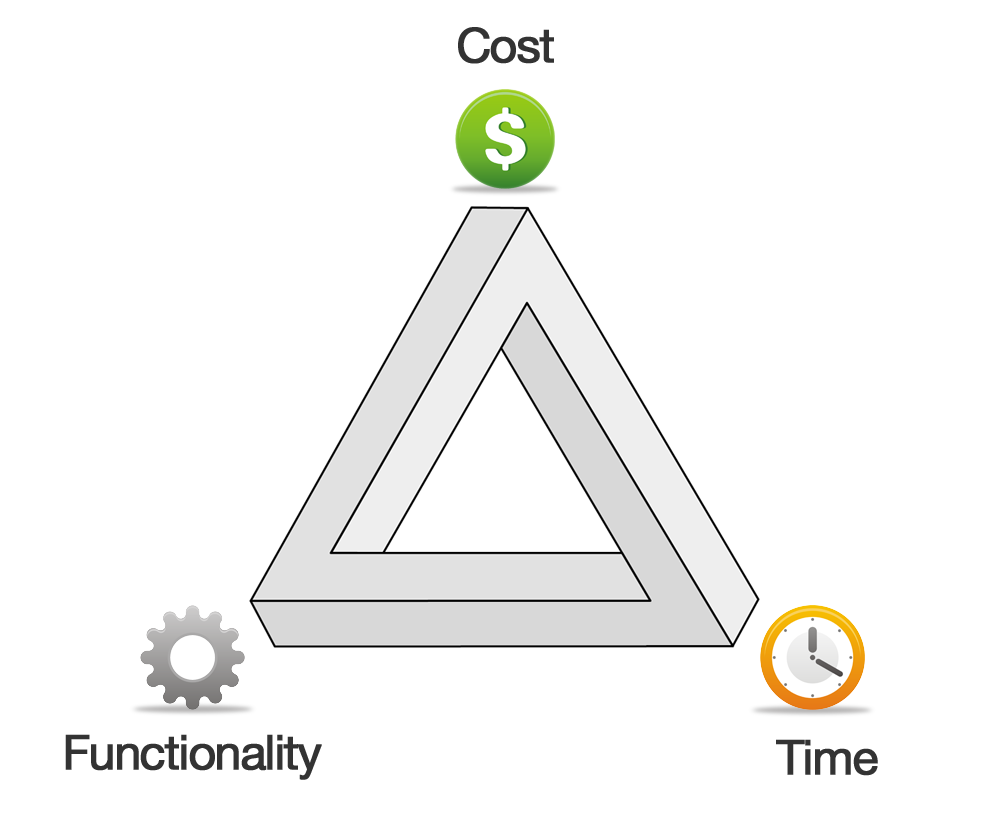
\includegraphics[scale=0.2]{figures/project_triangle.png}
\caption[Project management triangle]{Project management triangle \cite{website:claromentis}.}
\label{fig:project_triangle}
\end{figure}

\noindent
The cost of this student project is limited by its approved budget, a sum between 10,000 and 12,500 SEK, provided by \ac{LTU}. More funding can be applied for if required, but the budget nevertheless remains limited. This constraint implies a careful selection of components and the use of innovative engineering solutions throughout the entire project. 
\\
\\
The time available for this project is also constrained, being a student project that has to be realized in concurrence with other academic duties. The estimated time frame is therefore between 2 and 6 months for a first prototype capable of test flight.
\\
\\
The final resource is related to the previously mentioned functionality. With a limited number of team members that have limited expertise in the field of airships, the project has to be technically balanced, taking into account the capabilities of the members of the team.

\subsection{Environment}

The \ac{SPA} that will be developed during the \ac{U-SPACE} project finally has to be tested outdoors. Since the \ac{U-SPACE} project is being executed in the city of Kiruna during the spring, summer and early autumn, it is important to take the environmental conditions during this period of the year into account.  Some of the these conditions are listed below in table \ref{tab:environment}, using data for the month of May \cite{website:weatherspark} as a representation of the entire project period.

\begin{table}[H]
\centering
\caption{Environmental conditions}
\label{tab:environment}
\begin{tabular}{p{0.35\textwidth} p{0.15\textwidth} p{0.15\textwidth} p{0.35\textwidth}}
\hline
\textbf{Parameter} & \textbf{Lower boundary} & \textbf{Upper boundary} & \textbf{Remarks}\\ \hline
Temperature & -2 $^\circ$C & 11 $^\circ$C & Average values\\
Wind speed & 1 m/s & 6 m/s & Usually from the south west\\
Probability of precipitation & 61 \% & 61 \% & Average value\\
Hours of sunshine & 17:38 h & 22:45 h & Daily values\\
Cloud cover & 83 \% & 83 \% & Median value\\
Solar incidence angle at noon & 46 $^\circ$ & 46 $^\circ$ & Refer to document USPACE-PDR-PWR-A1\\
\hline
\end{tabular}
\end{table}

\subsection{Law}

The final constraints that have to be taken into account are possible legal issues that may arise during the construction and testing of the \ac{SPA}. A first legal constraint is the compliance to the \ac{ITU} Radio Regulations \cite{book:freqalloc} when using wireless connections. Secondly, when flying the \ac{SPA}, the Swedish Transport Agency's regulations on \ac{UAS} \cite{regulations:uas2009} might have to be taken into account. As these application of these regulations depends on the final mass and size of the prototype airship, this constraint can only be investigated when a prototype is constructed.

\section{Expected Functionality}
%What are the expected performances of the subsystem, as related to the requirements above? (maybe including some margins)

Based on the project goals set forth in section \ref{sec:goals} and taking into account the constraints discussed in the previous section, a realistic prediction of the functionality of the final product of the \ac{U-SPACE} project can be made. The expected functionality of the small-scale \ac{SPA} are summarized in table \ref{tab:expected}.

\begin{table}[H]
\centering
\caption{Expected functionality}
\label{tab:expected}
\begin{tabular}{c c c c}
\hline
\textbf{Parameter} & \textbf{Value} & \textbf{Remarks}\\ \hline
Autonomy & 2 h & At peak power\\
Flight altitude & 2-20 m & /\\
Forward velocity & 0.5-1 m/s & /\\
Flight conditions & Daytime & Sunny and calm weather\\
\hline
\end{tabular}
\end{table}

\noindent
The other functional constraints presented in section \ref{sec:constraints} will be discussed in subsequent chapters. In the future, this functionality might be expanded with features like autonomous attitude control and altitude control during flight.

\section{Fault Tolerance Design and Safety Concept}

Since the goal of the \ac{U-SPACE} project is to design, build and test a prototype of a small-scale \ac{SPA} the focus of this project is not on a fault-tolerant design of the airship, but rather on a performant design that meets the project goals. Nevertheless some safety features are included in the design, construction and flight test of the airship. These features will be discussed in the chapters dedicated to the different subsystems and in chapter \ref{chap:ground_support}.

\section{Materials}

With the limited time and funding inherent to this student-driven project great care needs to taken with regards to the selection and processing of the materials. The materials need to be as performant as possible for their specific function while at the same time their cost should be as low as possible. In general all materials should also be as light as possible. The specific material requirements for each subsystem are discussed in the subsequent chapters.
\\
\\
With regards to the processing of the materials, low cost is again the main discriminator to select an appropriate technique. Therefore the simplest techniques are preferred during the construction of the airship, with as less mechanical work as possible. A certain amount of experience with such techniques is present in the team, allowing short construction times and limited delays.
\newpage
\section{Critical Design}
\label{sec:critical_design}
%
This section describes in more detail the \ac{EPS} design. A simple block diagram of the \ac{EPS} design is shown in Figure \ref{fig:EPS_diagram_simple}.

\begin{figure}[H]
\centering
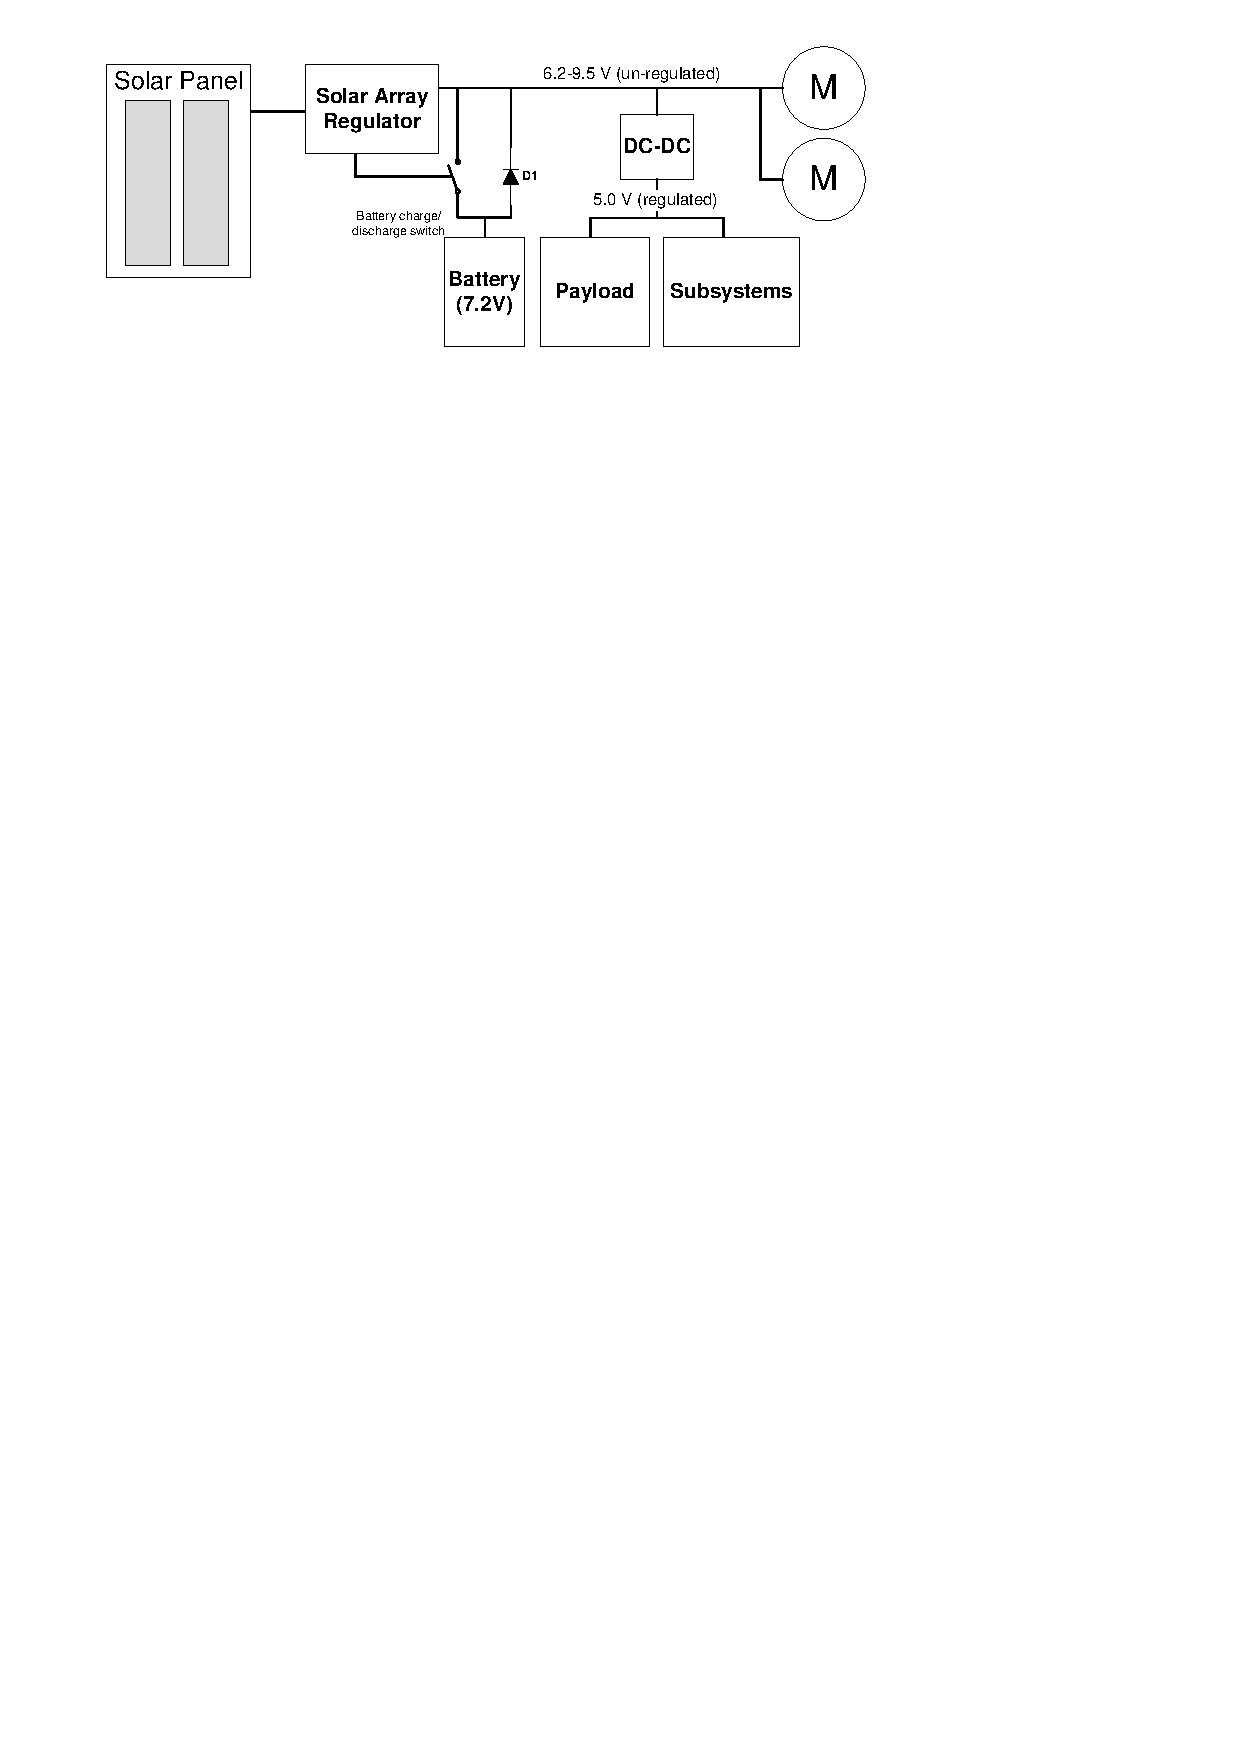
\includegraphics[width=\textwidth]{figures/fig_PDR_EPSdiagram}
\caption{\ac{EPS} simple blockdiagram}
\label{fig:EPS_diagram_simple}
\end{figure}
%
%
\subsection{Solar Array Design}
%Bypass diodes on SA to mitegate shadowing problems
%Cross-strapping of solar cells?
%\subsubsection*{Solar Array Shading}
%Bypass diodes can be used to partly mitigate this issue as well as using \ac{MPPT}. Otherwise it could be necessary to ensure that the airship structure cannot cast shadows on the panels and that the airship only fly above or away from landscape objects.
As was mentioned in section \ref{sec:changes_pdr_to_cdr}, a new solar cell has been selected. This solar cell is shown in Figure \ref{fig:solar_cell} and Table \ref{tab:solar_cell_spec} lists the important specifications for this cell.
%
\begin{figure}[H]
\centering
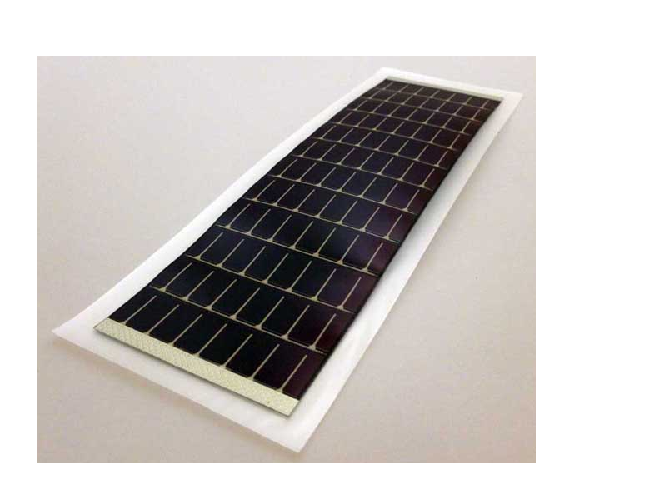
\includegraphics[width=0.3\textwidth]{figures/SolarCell_RC7-2_Powerfilm}
\caption{Chosen solar cell}
\label{fig:solar_cell}
\end{figure}
%
\begin{table}[H]
\centering
\caption{Specifications of chosen solar cell}
\label{tab:solar_cell_spec}
\begin{minipage}{\textwidth}
\begin{tabular}{ll}
\hline
Nominal output current & $100\,mA$\\
Nominal output voltage & $7.2V$\\
Nominal output power & $0.72\,W$\\
Dimensions & $270\,mm\:\times\:90\,mm\:\times\:0.2\,mm$\\
Weight & $7.6\,g$\\
No. of required cells $100$\footnote{\cite{avnetexpress} offers good discount for +100 units order}\\
Total solar panel area & $2.43\,m^2$ (assuming $100\,\%$ fill factor)\\
\hline
\end{tabular}\par
\vspace{-0.75\skip\footins}
\renewcommand{\footnoterule}{}
\end{minipage}
\end{table}
%
%
The solar panels will be configured with two series-connected solar cells thus having an output voltage of: 
%
\begin{equation}
V_{panel,out}=14.4\,V
\end{equation}
%
%
\subsection{Battery Design}
%
Two Panasonic PA-L60.K02 \cite{panasonic} Li-ion batteries are used. The battery has the following important specifications:
%
\begin{table}[H]
\centering
\caption{Specification of chosen battery}
\label{tab:proposed_battery}
\begin{tabular}{ll}
\hline
Chemistry & Li-ion\\
Nominal voltage & $3.6\,V$\\
Capacity & $1.03\,Ah$ / $3.61\,Wh$\\
Weight & $25\,g$\\
Dimensions & $56\,mm\:\times\:34.2\,mm\:\times\:5.8\,mm$\\
Maximum charge current & $970\,mA$\\
Maximum discharge current (continuous) & $1.455\,A$\\
\hline
\end{tabular}
\end{table}
%
%
\subparagraph*{Future Recommendations}
%
The chosen type of Li-ion battery supports only a relative low charge- and discharge rate of about $1\,C$. For bigger battery capacity and higher loads, it is recommended to use a battery like \cite{rcflight_battery} which provides much higher discharge rates ($>20\,C$) and also cheaper price per Wh. Only disadvantage  is a mass increase of around $15-25\%$.
%
\subsubsection{Battery Charge Regulator}
%
From the battery datasheet, maximum charge current is $I_{REG}=970\,mA$. From the \ac{BCR} datasheet, the minimum current sense resistor value is calculated as
%
\begin{equation}
\begin{split}
R_{sense}=&\dfrac{V_{FCS}}{I_{REG}}\\
R_{sense}=&\dfrac{120\,mV}{970\,mA}=123\,m\Omega
\end{split}
\end{equation}
%
The required thermal rating of the pass transistor is calculated as
%
\begin{equation}
P_{max}=(V_{in,max}-V_{bat,min})\cdot I_{charge}=(9.5\,V-5.5\,V)\cdot 970\,mA=3.88\,W
\end{equation}
%
\subsubsection{Battery Temperature Monitoring}
%
The \ac{BCR} chip includes a temperature monitoring feature. The battery is rated, in charge-mode, to temperature in the interval $10-45^{\circ}C$. The maximum allowed temperature is set slightly lower to $40^{\circ}C$. The Li-ion battery has a build-in \ac{NTC} thermistor with $B=3980\,K$ and $R_{25}=10k\,\Omega$. The required restance values of the temperature control resistors are determined from the \ac{BCR} chip datasheet as 
%
\begin{equation}
\begin{split}
R_{cold}&=R_{25}e^{B(\dfrac{1}{T}-\dfrac{1}{T_0}}=10\,k\Omega e^{3980\,K(\dfrac{1}{283	\,K}-\dfrac{1}{298\,K})}=20.3\,k\Omega\\
R_{hot}&=10\,k\Omega e^{3980\,K(\dfrac{1}{313	\,K}-\dfrac{1}{298\,K})}=5.3\,k\Omega\\
R_{T1}&=2\dfrac{R_{cold}R_{hot}}{R_{cold}-R_{hot}}=14.2\,k\Omega\\
R_{T2}&=2\dfrac{R_{cold}R_{hot}}{R_{cold}-3R_{hot}}=47.8\,k\Omega
\end{split}
\end{equation}

%
\subsubsection{Battery Discharge Current Limiter}
%
The selected MOSFET has a typical gate threshold voltage of $V_{Gth}=550\,mV$. The chosen \ac{BJT} has a typical collector-emitter voltage drop of $V_{CE}=120\,mV$. The battery is rated for a maximum discharge current of $I_{discharge}=1.455\,A$. The required current sense resistor is then calculated as 
%
\begin{equation}
\begin{split}
V_{sense}&=V_{Gth}-V_{CE}=550\,mV-120\,mV=430\,mV \Rightarrow\\
R_{sense}&=\dfrac{V_{sense}}{I_{discharge}}=\dfrac{430\,mV}{1.455\,A}=295\,m\Omega
\end{split}
\end{equation}
%
The exact required resistance must be determined by testing the precise parameters of the discrete components.
%
%
%
\subsection{Maximum Power Point Tracking Regulator}
%Which design concepts are considered? - What are the advantages/disadvantages for each concept?
%Decide on MPPT algorithm (using analog circuits?)
%DC-DC regulator topology (Buck, Boost, Buck-Boost etc.)
%
In \cite{PDR} it was decided to use a \ac{MPPTU} for the \ac{APR} due to its high efficiency and robustness to changing environmental constraints.

In first step, only the DC-DC converter will be implemented. When time and resources allows the \ac{MPPT} part will be added.
A simple buck DC-DC converter topology is used, comprising a transistor, free-wheel diode, inductor and output capacitor. 
When the full \ac{MPPTU} is implemented, it will operate in three different operation regions:
%
\begin{itemize}
\item Battery discharge {MPPT} - when the solar array input power is insufficient to cover the load power demand, the battery is slowly discharged in order to maintain the output voltage.
\item Battery charge {MPPT} - when the solar array input is greater than the load power, the excessive power is used to recharge the battery.
\item Input power limitation - when the battery is fully charged, the regulator will operate the solar array at a non-optimal voltage, thus limiting the input power to keep the output voltage constant. The extra potential input power is dissipated as heat externally on the solar arrays.
\end{itemize}
%
\begin{figure}[H]
\centering
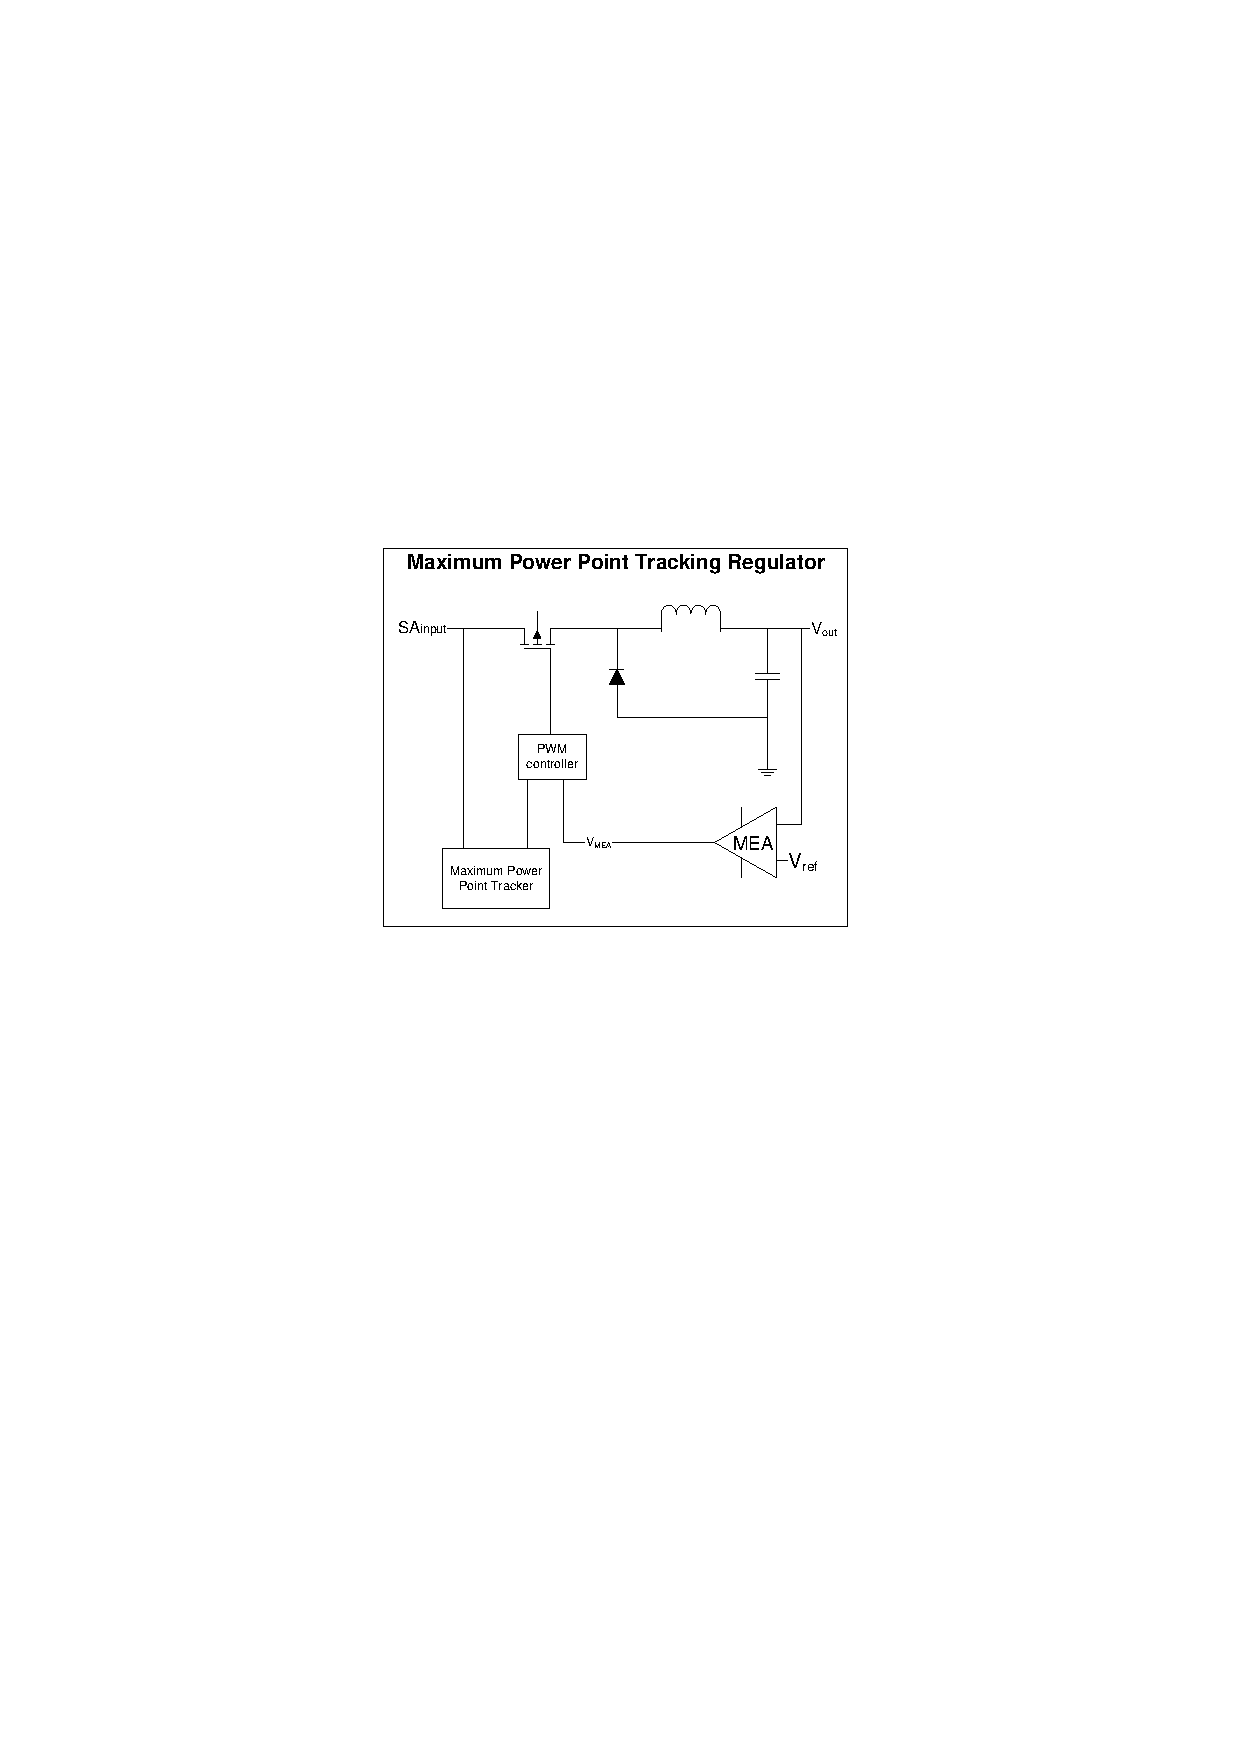
\includegraphics[scale=1]{figures/fig_PDR_MPPTdiagram}
\caption{\ac{MPPT} regulator diagram}
\label{fig:MPPT_regulator}
\end{figure}
%


\subsubsection{Mainbus Under Voltage Protection}
%
The power from battery and solar cells is limited. It is thus possible that the motors will try to draw more current than what can be delivered. If this happens, the output capacitor of the \ac{APR} will quickly discharge and the main output voltage drops out. To prevent this situation, an \ac{UVP} circuit is added. This is implemented using an $STN888$ PNP \ac{BJT} along with two resistors, $R3$ and $R4$ as shown in Figure \ref{fig:EPS_diagram_detailed}. When the main output voltage is around $6.2\,V$ the Base-Emitter voltage drop is close to $1.2\,V$ and the \ac{BJT} is fully conducting and effectively works as a short circuit. If the output voltage drops significantly below $6.2\,V$ the \ac{BJT} will begin to decrease the output current until the output voltage stabilizes. The current gain of $STN888$ is about $100$, hence to allow an maximum output current of $10\,A$, the resistors $R3$ and $R4$ must be designed to pass $100\,mA$ at $6.2\,V$ output voltage. To minimize efficiency it is important that the forward voltage drop of the \ac{BJT} is kept as low as possible.

\subparagraph*{Further Recommendations}
%
It is hard to find suitable \acp{BJT} rated for much more than $5\,A$. If the power output is increased in future designs, it is suggested to either parallel connect several \acp{BJT} however this might cause issues with thermal runaway. Alternatively high current \acp{IGBT} can be used, however they have higher forward voltage drops and thus they are more suitable for a design with a higher output voltage.


%
\subsection{Complete EPS Diagram}
%
The complete \ac{EPS} diagram is shown in Figure \ref{fig:EPS_diagram_detailed}. For providing the $5\,V$ regulated voltage to the payloads, \ac{COTS} DC-DC regulator(s) are used. The battery charging/discharging is controlled by the \ac{SAR}.
%
\begin{sidewaysfigure}
\centering
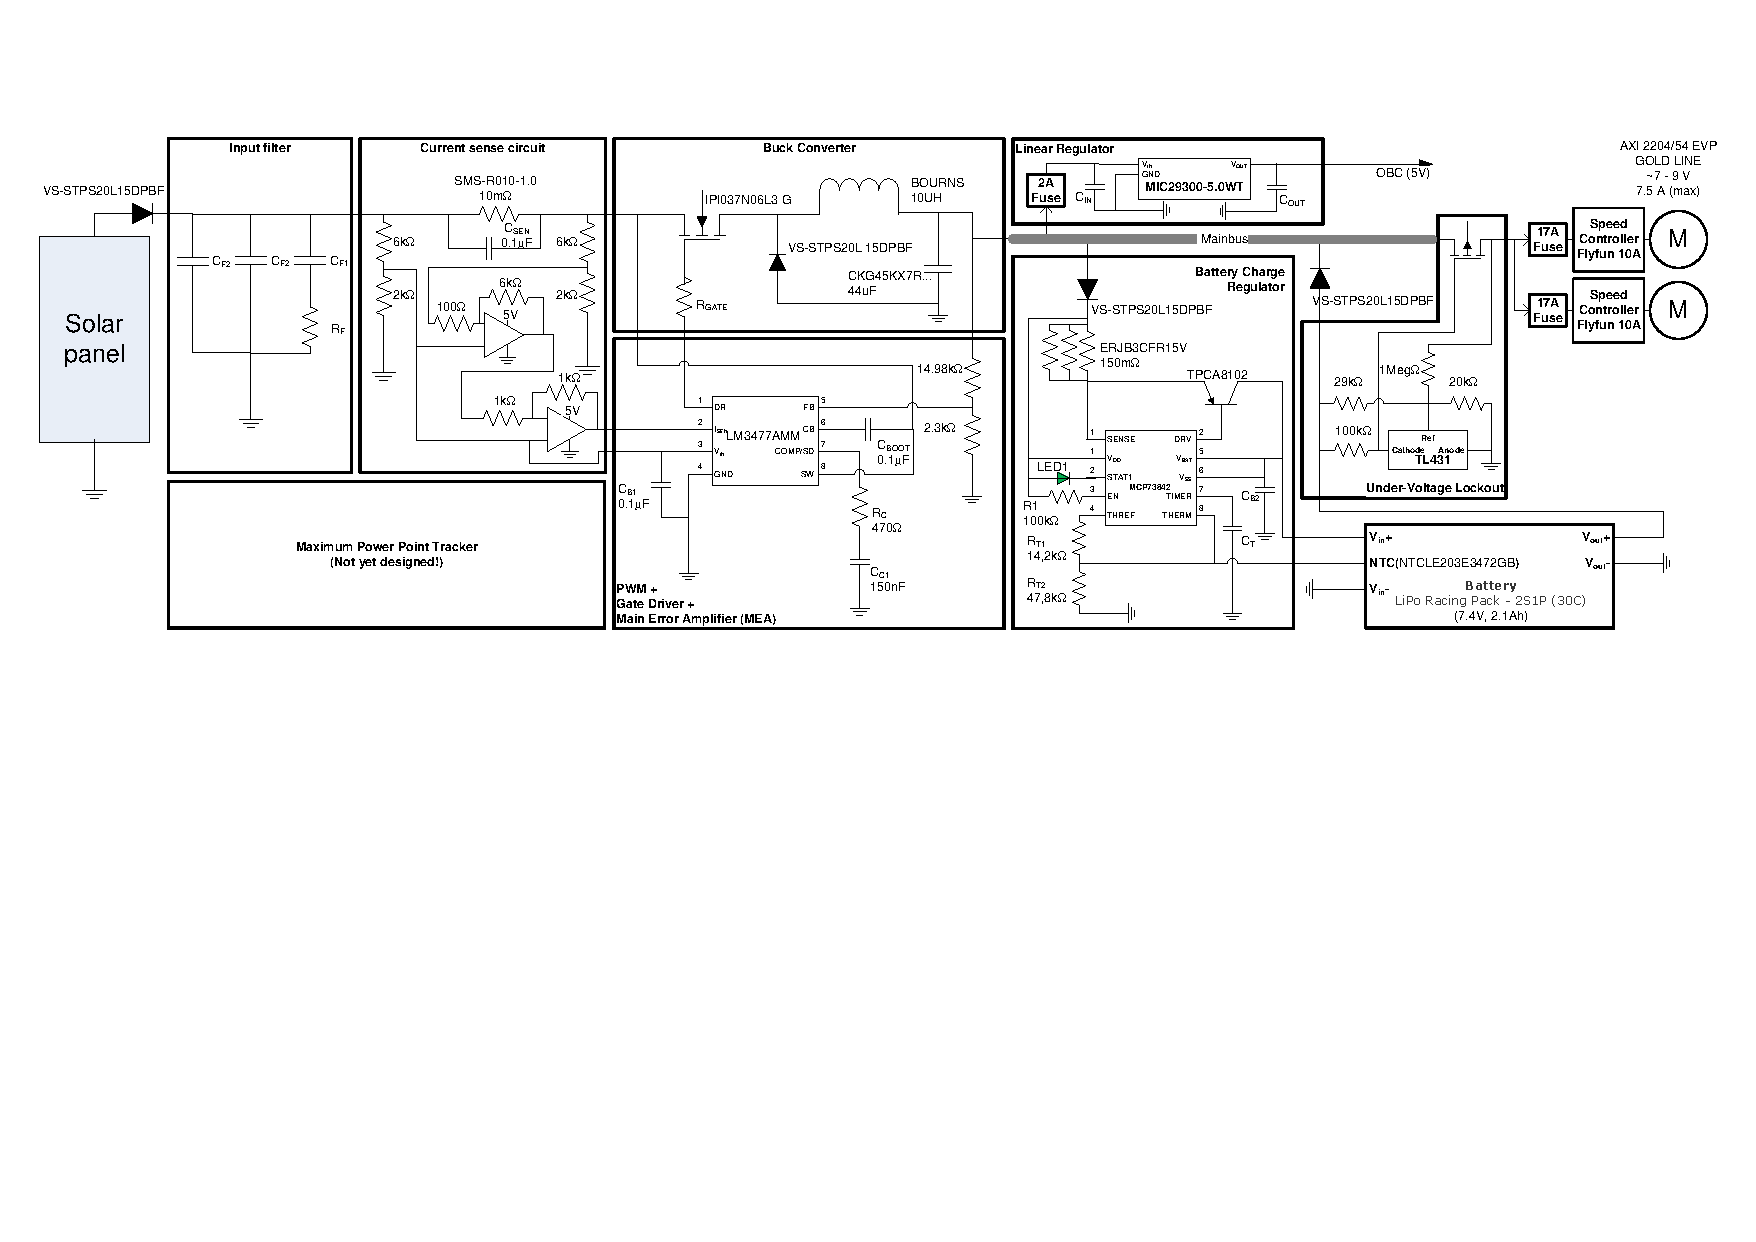
\includegraphics[scale=0.8]{figures/fig_CDR_EPSdiagram_detailed}
\caption{\ac{EPS} detailed block diagram diagram}
\label{fig:EPS_diagram_detailed}
\end{sidewaysfigure}

%
\subsection{External Interfaces}
%
The interfaces of the \ac{EPS} external are listed in table \ref{tab:external_interfaces}.
%
\begin{table}[H]
\centering
\caption{External interfaces}
\label{tab:external_interfaces}
\begin{tabular}{m{0.35\textwidth}m{0.55\textwidth}}
\hline
\textbf{External interface} & \textbf{Implementation}\\
\hline
Solar cells mounting & \ac{PSA}\\[2mm]
DC-DC regulators & Mounted on PCB which sits in system housing. Thermal contact points should be included, to remove internal heat dissipation.\\[2mm]
Battery telemetry & Analog signals to Microcontroller\\[2mm]
Mounting of batteries & \ac{TBD}\\
%Output voltage control(reference voltage setpoint) & Analog signal from Microcontroller\\[2mm]
Supply voltages & $6.0-9.2\,V$ (unregulated) and $5.0\,V$(regulated)\\[2mm]
\hline
\end{tabular}
\end{table}
%
%
\subsection{Telemetry and Telecommands}
%What telemetries/telecommands are required/useful for the subsystem? – What data rates/sizes are required?
%
The required/recommended telemetry and telecommands, \ac{EPS} , are listed in table \ref{tab:Telemetry_Telecommands}.
%
\begin{table}[H]
\centering
\caption{Telemetry and telecommands}
\label{tab:Telemetry_Telecommands}
\begin{tabular}{|l|l|l|}
\hline
\textbf{Telemetry} & \textbf{Data rate/frequency} & \textbf{Data size} \\
\hline
Battery voltage & Every 30 sec & 2 bytes\\
\hline
Battery temperature & Every 5 sec & 2 bytes\\
\hline
%Solar array temperature & Every 30 sec & 1 byte\\
%\hline
%Solar array voltage & Every 1 sec(MPPT performance) & 2 bytes\\
%\hline
%Solar array current & Every 1 sec(MPPT performance) & 2 bytes\\
%\hline
\end{tabular}
\end{table}
\section{Test and Verification of Design}
\label{sec:test_verification}
This section describes the various design models used to develop the \ac{EPS} along with the expected functional test to be executed.
%
\subsection{EPS Design Models}
%
\subsubsection{EPS PSpice Simulations}
A transient PSpice simulation model of the whole \ac{EPS} is currently being implemented. The completed PSpice models are shown in Appendix \ref{app:EPS_PSpice}. These will help in the design and testing of the regulator performance and system stability during transient loading as well as the interactions between the different circuits.

In future, it is desired also to implement transient PSpice models for the solar array\cite{Castaner}, \ac{MPPTU}, battery\cite{gold}, motors and \ac{BCR}.
%
\subsubsection{EPS Development Model}
An \ac{EPS} \ac{DM} is currently being build as seen in Figure \ref{fig:EPSprototype}. The prototype \ac{PCB} is realized using self-made "mini-mount" \ac{PCB} pads as shown in Appendix \ref{app:EPS_mini-mount}. These pads are attached, using a simple glue roller, on a complete copper ground plane. This design approach allows a compact layout which reduces parasitic effects. Also any \ac{IC} package can be supported and parts can easily be moved around if the design changes.
%
\begin{figure}[H]
\centering
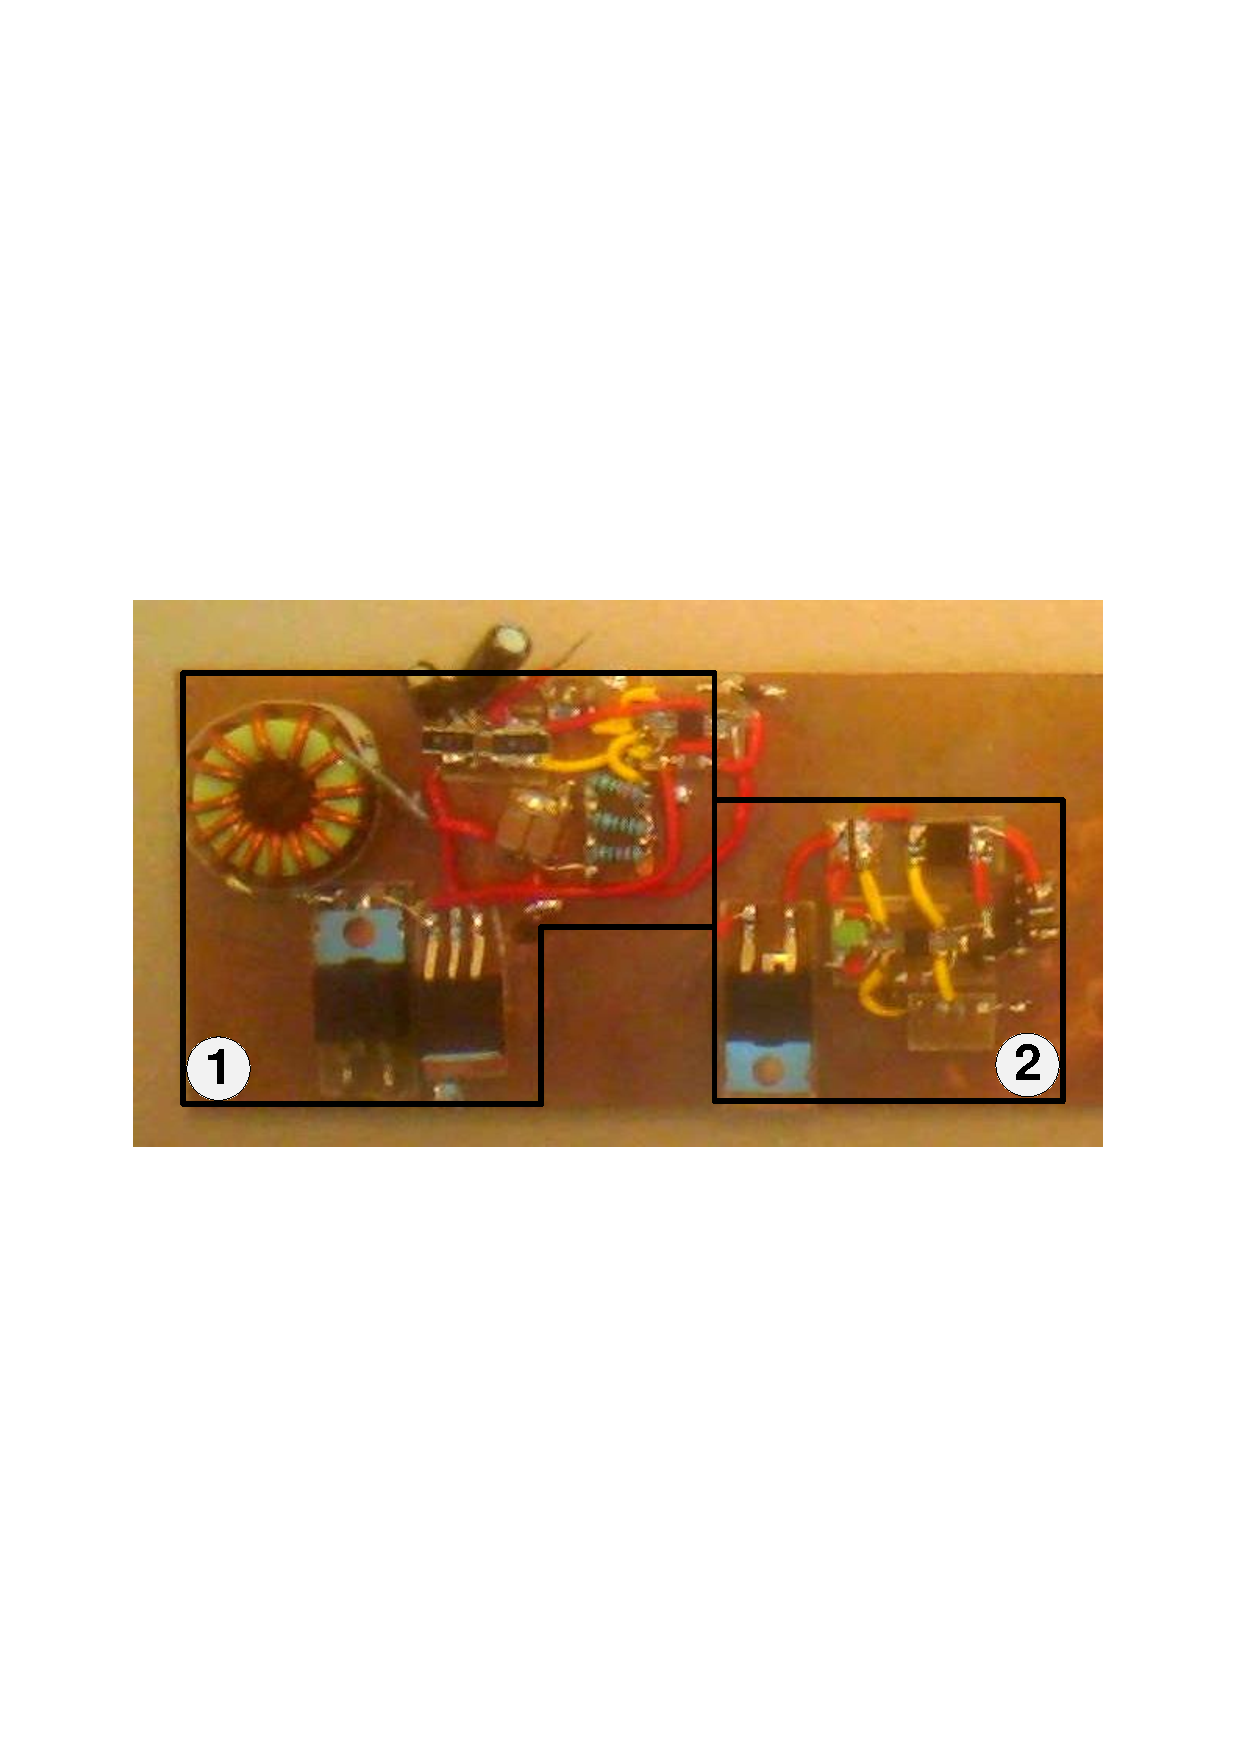
\includegraphics[width=0.8\textwidth]{figures/fig_CDR_EPSprototype}
\caption{\ac{EPS} prototype - \textbf{1}:\ac{SAR}, \textbf{2}:\ac{BCR}}
\label{fig:EPSprototype}
\end{figure}
%
\subsubsection*{Development Model Status}
The \ac{SAR} is working but shows signs of \ac{CM} instability which is expected to be caused by the missing current sense amplifier circuit and input filter. Development progress is currently awaiting delivery of components.

The \ac{BCR} is also working however excessive heating of the MOSFET was experienced. A new part rated for higher power dissipation has been selected and is currently awaiting delivery.
%
\subsubsection{EPS Flight Model}
If time allows, a dedicated \ac{FM} will be build, using a custom designed \ac{PCB} schematic layout. An optimized \ac{PCB} layout will minimize the system mass and size while maximizing the efficiency and system robustness.
%
\subsection{EPS Test Program}
Table \ref{tab:test_program} lists all necessary and desired test of the EPS. Priority "1" tests are all required while priority "2" tests will only be realized if time and resources allow it.
%
\begin{center}
\begin{longtable}[H]{p{0.15\textwidth}p{0.3\textwidth}p{0.45\textwidth}r}
\caption{EPS Test Program}\\
\label{tab:test_program}\\[-0.5cm]
\hline
\textbf{Subsystem} & \textbf{Condition/Mode} & \textbf{Test Description} & \textbf{Pri.}\\
\hline
\ac{SAR} & Mainbus voltage limitation & With more input power than load power, \ac{SAR} must be able to maintain a stable $9.5\,V$ output voltage also during transient loading & 1\\
- & Maximum power handling & With an input and load power slightly above the maximum expected solar array power, no \ac{SAR} components must overheat or otherwise malfunction & 1 \\
- & \ac{MPPT} & \ac{TBD} & 2\\
- & Mode transitions & \ac{SAR} must be able to change between \ac{MPPT}, battery charge and discharge mode without loosing mainbus voltage regulation or causing other malfunctions & 2\\
- & Feedback loop stability & Regulator bandwidth, gain- and phase margins should be measured with a Network Analyzer & 2\\
- & \ac{EMC} & Electromagnetic emissions should be measured with a Spectrum Analyzer, especially with concerns to the telecommunication systems & 2\\
\hline
\ac{BCR} & \ac{CC} and trickle charging & \ac{CC} charge at $2.4\,A$ and trickle charge mode entered when battery voltage reaches $8.4\,V$ should be verified & 1\\
- & Charge inhibit at high/low temperatures & While battery is charging, battery thermistor is heated/cooled in thermal oven/fridge to slightly above/below the specified temperature limits and charging should be terminated & 1\\
\hline
\ac{UVLO} & Power cut-off and recovery & Reducing input voltage below calculated threshold voltage should open switch and switch should close again when input voltage is increased above the threshold & 1\\
\hline
Battery & Dynamic model & Test approach is described in \cite{chen} & 2\\
\hline
Solar cell & I-V specifications & short-circuit current, open-circuit voltage, current and voltage at the \ac{MPP} should be determined from an irradiance test & 2\\
- & Temperature coefficients & Solar cell temperature coefficients should be determined be measuring the I-V characteristics at different temperatures within the expected temperature interval & 2\\
\hline
Fuses & Temperature variation & The \ac{PTC} resettable fuses should be tested at nominal, minimum and maximum expected temperatures to verify acceptable functionality & 1\\
\hline
\end{longtable}
\end{center}
%
\section{Resources and Scheduling}
\label{sec:resources_scheduling}

\subsection{Main Tasks}
some text...

\subsection{Parts List and Costs}
some text...

\subsection{Electronics Ground Support Equipment (EGSE)}
some text...

\subsection{Mechanical Ground Support Equipment (MGSE)}
some text...

\newpage
\printbibliography
\markboth{Bibliography}{Bibliography}
\addcontentsline{toc}{section}{\protect\numberline{}References}
\newgeometry{margin=1.5cm}
\pagestyle{plain}

%\appendix

\chapter{Some Appendix}\label{app:SomeAppendix}
some text...

\chapter{Another Appendix}\label{app:AnotherAppendix}
some text...

\end{document}